\documentclass[journal]{IEEEtran}

% *** CITATION PACKAGES ***
\usepackage[style=ieee]{biblatex} 
\bibliography{random_walk.bib}    %your file created using JabRef

% *** MATH PACKAGES ***
\usepackage{amsmath}

% *** PDF, URL AND HYPERLINK PACKAGES ***
\usepackage{url}
\hyphenation{op-tical net-works semi-conduc-tor}
\usepackage{graphicx}  %needed to include png, eps figures
\usepackage{float}  % used to fix location of images i.e.\begin{figure}[H]

% *** MY PACKAGES ***
\usepackage{todonotes}


\begin{document}

% paper title
\title{Using Random Walk Simulations to Calculate Ground State Energies in Quantum Physics}

% author names 
\author{Sai Pandian, ID: 29899923}% <-this % stops a space
        
% The report headers
\markboth{PHYS6017 Computer Techniques in Physics Report 1, April 2020}
{Shell \MakeLowercase{\textit{et al.}}: Bare Demo of IEEEtran.cls for IEEE Journals}

% make the title area
\maketitle

% As a general rule, do not put math, special symbols or citations
% in the abstract or keywords.
\begin{abstract}
Provide a summary of the session. What was done, what measurements were taken,
brief methods, what calculations, brief conclusion.  The Abstract should be
approximately 250 words or fewer, italicized, in 10-point Times (or Times
Roman.) Please leave two spaces between the Abstract and the heading of your
first section.  It should briefly summarize the essence of the paper and address
the following areas without using specific subsection titles. Objective: Briefly
state the problem or issue addressed, in language accessible to a general
scientific audience. Technology or Method: Briefly summarize the technological
innovation or method used to address the problem. Results: Provide a brief
summary of the results and findings. Conclusions: Give brief concluding remarks
on your outcomes. Detailed discussion of these aspects should be provided in the
main body of the paper.
\end{abstract}

\begin{IEEEkeywords}
keywords, temperature, xxxx equation, etc.
\end{IEEEkeywords}

\section{Introduction}
% Here we have the typical use of a "W" for an initial drop letter
% and "RITE" in caps to complete the first word.
% You must have at least 2 lines in the paragraph with the drop letter
% (should never be an issue)

\IEEEPARstart{R}{andom} walks are a simple model of motion in which a path is
described as a succession of steps with each step being in a random direction on
some vector space. Random walks are useful in modelling many physical processes
that are perceived as having a pseudo-random mechanism \todo{cite}. Their
applications range from Biology to the Stock Market. This paper aims to explore
how Random Walk Simulations can be implemented to calculate the ground state
energies of different quantum systems. \todo{more}

\section{Theoretical Background}

Random walks work descibe motion as a series of steps, with the direction of
each step being random. Figure \ref{fig:cartoon} demonstrates this concept by
considering a one-dimensional line. On this line, the ``walker'' starts at the
origin, and walks a total of 20 steps. The walker at each step has a equal
chance of stepping forwards, or stepping backwards.

\begin{figure}%[H]%[!ht]
  \begin{center}
    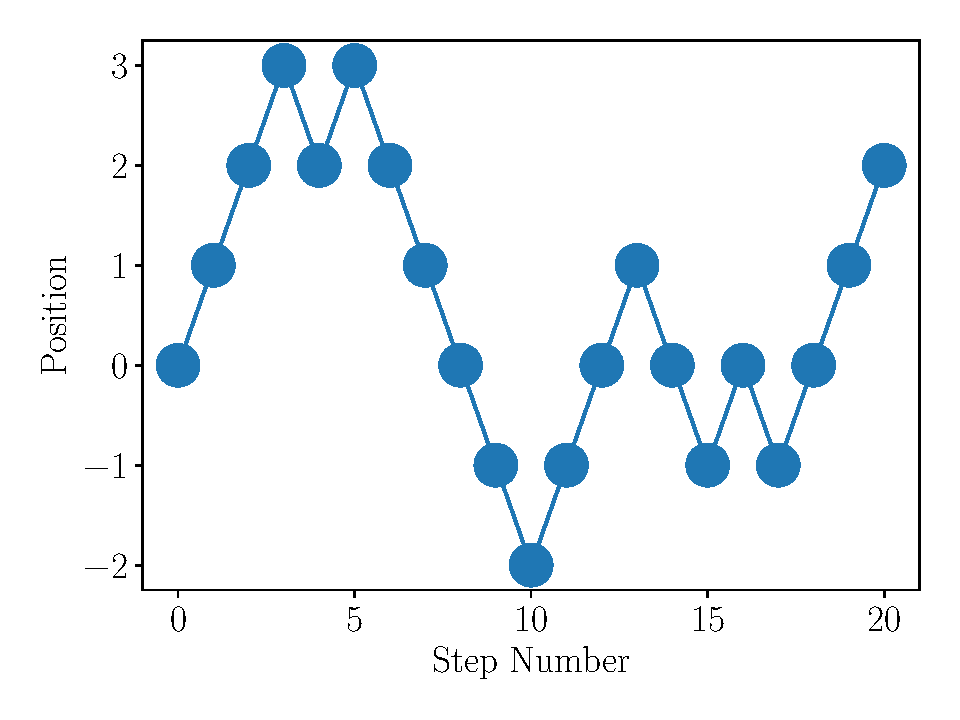
\includegraphics[width=0.45\textwidth]{images/cartoon.pdf}
    \caption{Illustrations, graphs, and photographs may fit across both columns, if necessary. Your artwork must be in place in the article.}
    \label{fig:cartoon}
  \end{center}
\end{figure}

As can be seen from the figure, it is not uncommon for the average position of
the walker to be away from the origin once the walk has concluded. This is
because the position of the walker at any step is dependent only on the position
at the previous step. If the walker happens to take a number of steps in the
same direction, it is highly unlikely for the walker to take an equal number of
steps in the opposite direction, in order to return to the origin. Thus, in such
a case, it is likely that the walker will conclude the walk in a position away
from the origin.

In this example, the walker had an equal likelihood of stepping forward or
backwards, but we can bias in one way if we want to model a particular
phenomenon. The walk is also easily extensible to multiple dimensions, as for
each extra dimension, one extra random number must be drawn. This gives a linear
increase in time-complexity, which is convenient for long computations.

Random Walk simulations can be applied to calculate the ground state energies of
Quantum Systems by solving the Schr\"{o}dinger equation. Consider a
one-dimensional simple lattice system. A walker can start at a position labelled
the origin, and then proceed in a random walk. The random walk concludes after a
certain number of steps or if the walker ``dies'' on a particular step. The
probability that the walker will die is dependent on a defined potential at that
point. For example, in an infinite square well system, the potential is 0 within
a well, and infinite outside the well. So the walker will have no chance of
dying whilst inside the well, but will die if they step outside.

Let us define $p(j,n)$ as the probability that the walker will be at position
$j$ after $n$ steps and $a(j)$ as the probability that the walker will die at
position $j$. If we say:

\begin{equation}
  p(j,n) = q(j) exp(-\lambda n)
  \nonumber
\end{equation}
where $q(j)$ is an arbitrary function and $\lambda$ is the rate of death, then:
\begin{equation}
  -\frac{1}{2} \frac{d^2q(j)}{dj^2} + a(j)q(j) = \lambda q(j)
  \nonumber
\end{equation}

\section{Results and Discussion}

Sample Text

\begin{figure}[H]%[!ht]
  \begin{center}
    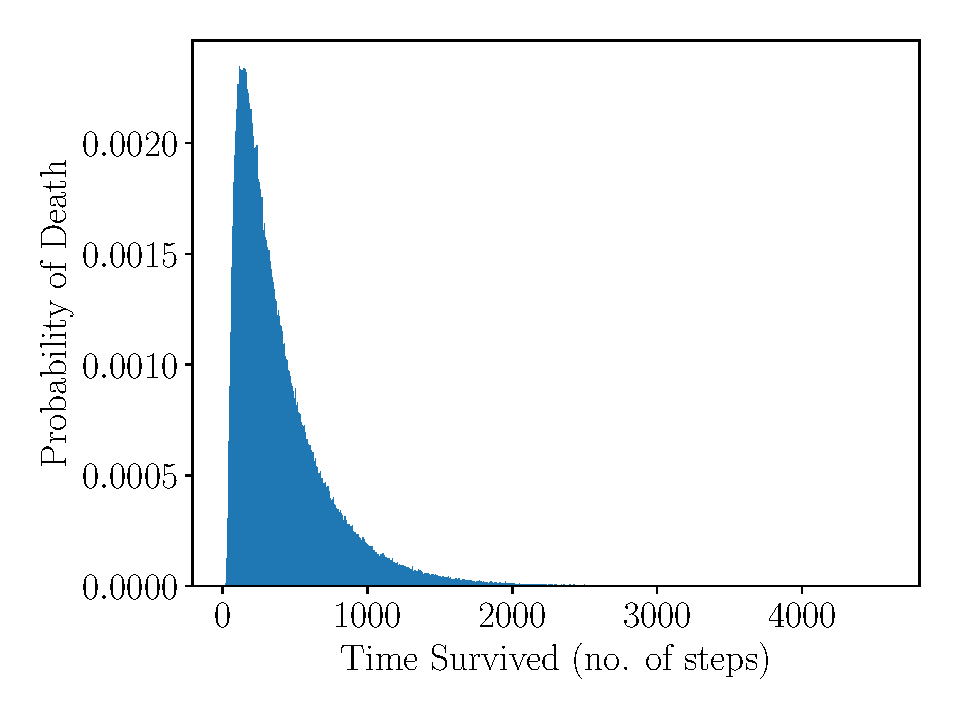
\includegraphics[width=0.45\textwidth]{images/exp_plot.pdf}
    \caption{Illustrations, graphs, and photographs may fit across both columns, if necessary. Your artwork must be in place in the article.}
    \label{fig:exp_plot}
  \end{center}
\end{figure}


\begin{figure}[H]%[!ht]
  \begin{center}
    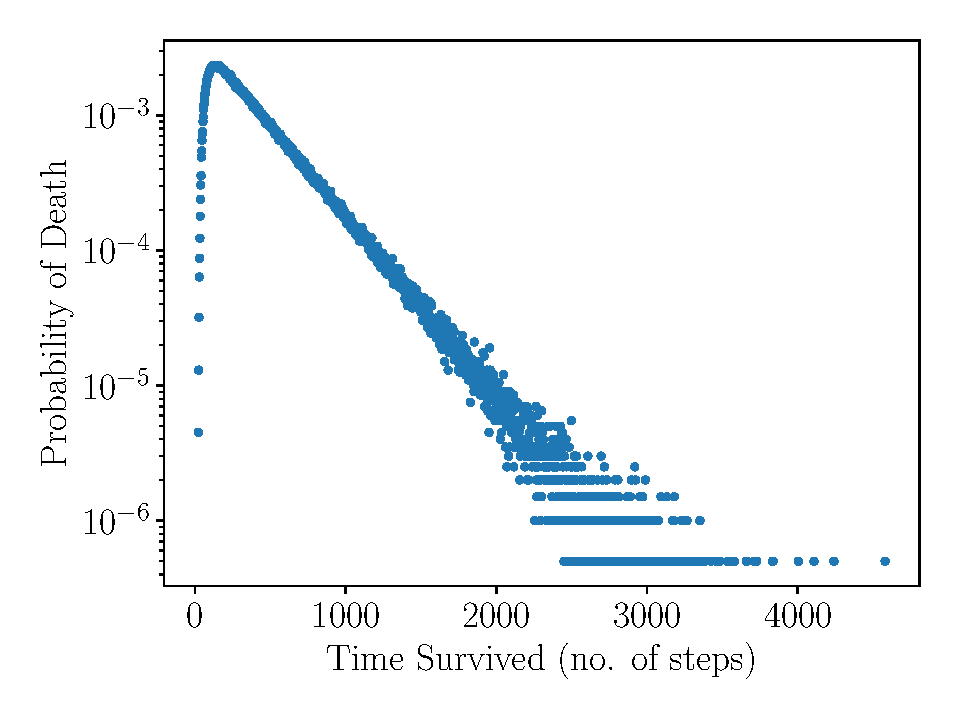
\includegraphics[width=0.45\textwidth]{images/line_plot.pdf}
    \caption{Illustrations, graphs, and photographs may fit across both columns, if necessary. Your artwork must be in place in the article.}
    \label{fig:line_plot}
  \end{center}
\end{figure}


\begin{figure}[H]%[!ht]
  \begin{center}
    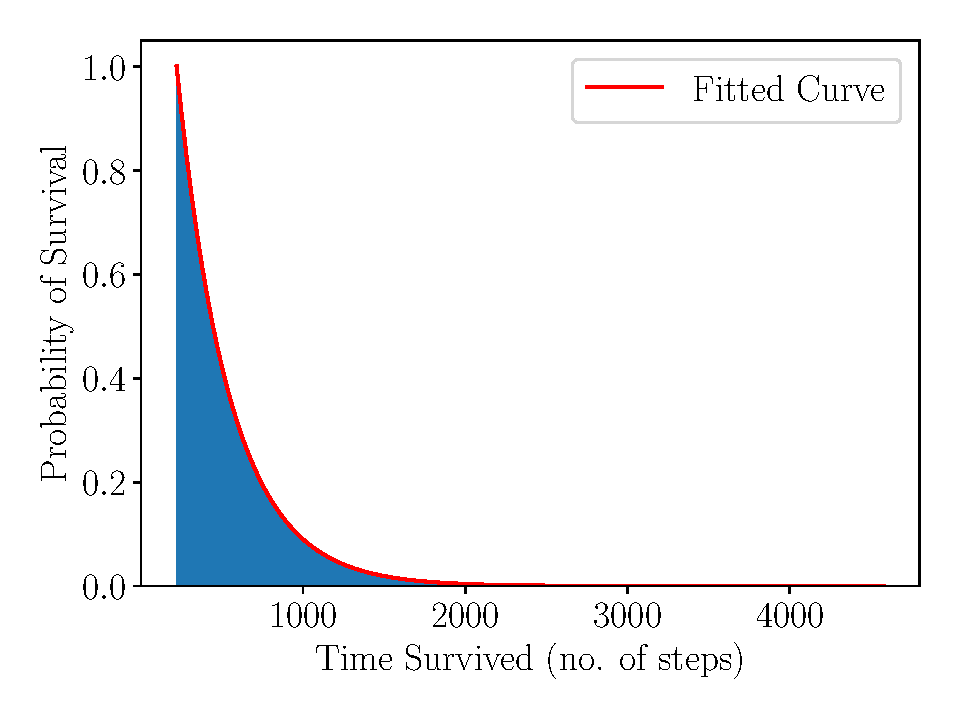
\includegraphics[width=0.45\textwidth]{images/cum_exp_plot.pdf}
    \caption{Illustrations, graphs, and photographs may fit across both columns, if necessary. Your artwork must be in place in the article.}
    \label{fig:cum_exp_plot}
  \end{center}
\end{figure}


\begin{figure}[H]%[!ht]
  \begin{center}
    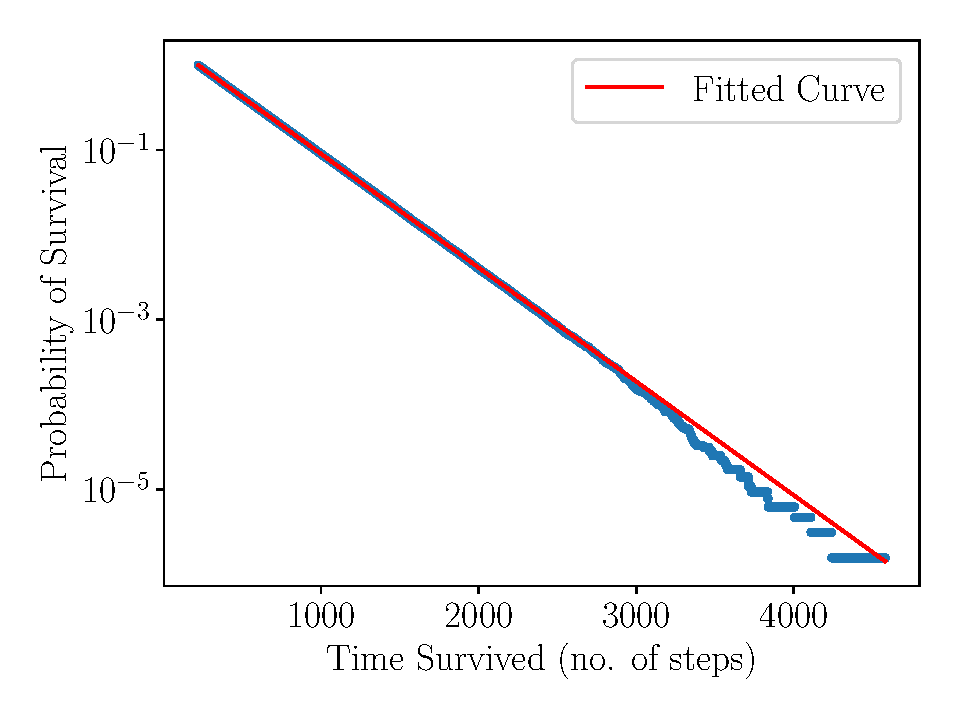
\includegraphics[width=0.45\textwidth]{images/cum_line_plot.pdf}
    \caption{Illustrations, graphs, and photographs may fit across both columns, if necessary. Your artwork must be in place in the article.}
    \label{fig:cum_line_plot}
  \end{center}
\end{figure}


\begin{figure}[H]%[!ht]
  \begin{center}
    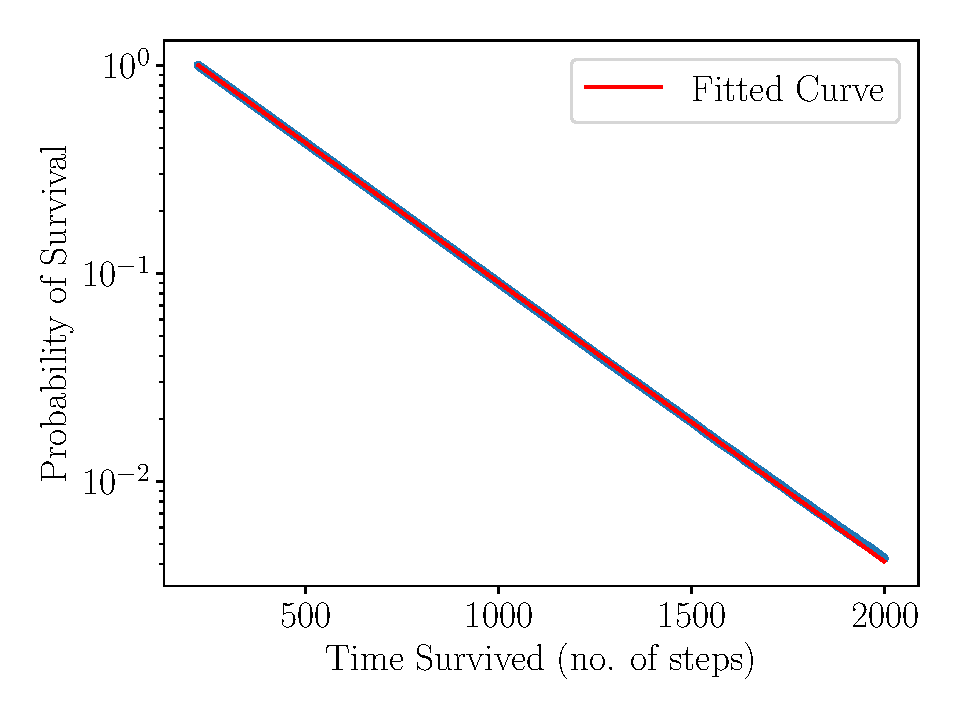
\includegraphics[width=0.45\textwidth]{images/cum_line_plot_cutoff.pdf}
    \caption{Illustrations, graphs, and photographs may fit across both columns, if necessary. Your artwork must be in place in the article.}
    \label{fig:cum_line_cutoff_plot}
  \end{center}
\end{figure}

\section{Conclusions}

Sample Text


% if have a single appendix:
%\appendix[Proof of the Zonklar Equations]
% or
%\appendix  % for no appendix heading
% do not use \section anymore after \appendix, only \section*
% is possibly needed

% use appendices with more than one appendix
% then use \section to start each appendix
% you must declare a \section before using any
% \subsection or using \label (\appendices by itself
% starts a section numbered zero.)
%



\appendices
\section{Random Walk Schr\"{o}dinger Equation Derivation}
Let us denote the probability that the walker is at position $j$ after $n$ steps
as $p(j,n)$ and the probabilty that the walker will die at position $j$ as
$a(j)$. We will denote the position-step number coordinates as $[j, n]$. Thus,
for a walker to have coordinates $[j, n+1]$, in the previous step, they must have
had coordinates $[j \pm 1, n]$. So we can say:

\begin{equation}
  \label{eq:probability}
  p(j, n+1) =  \frac{1}{2}(1-a(j))(p(j-1,n) + p(j+1,n))
\end{equation}

If $a(j)$ is small and $n$ is large, then we can say $p(j, n)$ is a continuous
function and we can use Taylor expansion to expand each of $p(j+1, n)$,
$p(j-1,n)$, and $p(j, n+1)$:

\begin{equation}
  p(j+1, n) = p(j,n) + \frac{\partial p}{\partial j} + \frac{1}{2}
  \frac{\partial^2 p}{\partial j^2} + ...
  \nonumber
\end{equation}
\begin{equation}
  p(j-1, n) = p(j,n) - \frac{\partial p}{\partial j} + \frac{1}{2}
  \frac{\partial^2 p}{+\partial j^2} + ...
  \nonumber
\end{equation}
\begin{equation}
  p(j, n+1) = p(j, n) + \frac{\partial p}{\partial n} + ...
  \nonumber
\end{equation}

We can now substitute these expansions into Equation \ref{eq:probability}, we
find:

\begin{equation}
  p(j, n) + \frac{\partial p}{\partial n} = (1-a(j))\Big(p +
  \frac{1}{2}\frac{\partial^2 p}{\partial j^2}\Big)
  \nonumber
\end{equation}

But the probability of death $a(j)$ and the second derivative are so small, that
their product is neglected. We also let $p(j,n) = q(j) exp(-\lambda n)$ so that:


\begin{equation}
  item
  \nonumber
\end{equation}

% use section* for acknowledgment
\section*{Acknowledgment}
The authors would like to thank...

\printbibliography

% that's all folks
\end{document}


